\documentclass[aspectratio=169,11pt]{beamer}

\usepackage{graphicx}
\usepackage{tikz}
\usetikzlibrary{positioning,arrows.meta}
\usepackage{xcolor}
\usepackage{booktabs}
\usepackage{tabularx}
\usepackage{array}
\usepackage{ragged2e}

\definecolor{GEUBlue}{RGB}{20,55,105}
\definecolor{GEULightBlue}{RGB}{238,244,251}
\definecolor{GEUGrey}{RGB}{90,90,90}
\definecolor{GEULightGrey}{RGB}{245,246,248}

\usetheme{default}
\setbeamertemplate{navigation symbols}{}
\setbeamertemplate{blocks}[rounded][shadow=false]
\setbeamercolor{normal text}{fg=black,bg=white}
\setbeamercolor{frametitle}{fg=GEUBlue}
\setbeamercolor{structure}{fg=GEUBlue}
\setbeamercolor{block title}{fg=GEUBlue,bg=GEULightBlue}
\setbeamercolor{block body}{fg=black,bg=GEULightBlue}
\setbeamerfont{frametitle}{size=\Large,series=\bfseries}

% Replace with the actual logo filename
\newcommand{\GEULogo}{graphicera_logo.png}

% Header and footer
\setbeamertemplate{headline}{%
  \begin{tikzpicture}[remember picture,overlay]
    \node[anchor=north east,xshift=-0.30cm,yshift=-0.12cm]
      at (current page.north east)
      {\includegraphics[height=0.62cm]{\GEULogo}};
  \end{tikzpicture}
  \vspace{0.72cm}
}
\setbeamertemplate{frametitle}{%
  \vspace{0.03cm}
  \insertframetitle\par
  \vspace{0.04cm}
  \textcolor{GEUBlue}{\rule{\textwidth}{0.9pt}}
  \vspace{0.03cm}
}
\setbeamertemplate{footline}{%
  \leavevmode
  \hbox{%
  \begin{beamercolorbox}[wd=.82\paperwidth,ht=0.32cm,dp=0.10cm,leftskip=.3cm]{author in head/foot}
    \tiny Department of Computer Science \& Engineering | Graphic Era (Deemed to be University)
  \end{beamercolorbox}%
  \begin{beamercolorbox}[wd=.18\paperwidth,ht=0.32cm,dp=0.10cm,rightskip=.3cm]{date in head/foot}
    \hfill\tiny\insertframenumber/\inserttotalframenumber
  \end{beamercolorbox}}
}

\newcommand{\smallnote}[1]{\vspace{0.08cm}{\scriptsize\color{GEUGrey}#1}}
\newcommand{\placeholder}[1]{\textit{\color{GEUGrey}#1}}

\title{\textbf{Project-Based Learning}\\[2mm]\large Phase-I Evaluation}
\author{\textbf{Project Title}\\Team ID: XXXX}
\institute{Department of Computer Science \& Engineering\\Graphic Era (Deemed to be University), Dehradun}
\date{Academic Session 2026--27}

\begin{document}

% 1
\begin{frame}[plain]
\begin{tikzpicture}[remember picture,overlay]
\draw[GEUBlue,line width=3pt] (current page.north west) -- (current page.north east);
\node[anchor=north east,xshift=-0.45cm,yshift=-0.35cm] at (current page.north east)
{\includegraphics[height=1.0cm]{\GEULogo}};
\node[align=center,text width=.84\paperwidth] at ([yshift=.25cm]current page.center)
{{\color{GEUBlue}\fontsize{26}{30}\selectfont\bfseries PROJECT-BASED LEARNING}\\[3mm]
 {\fontsize{18}{22}\selectfont PHASE-I EVALUATION}\\[7mm]
 {\color{GEUGrey}\Large\bfseries \placeholder{TapNGo - A Bus Fare Verification And Payment System}}\\[3mm]
 {\color{GEUBlue}\normalsize Team ID: DSCPP-III-2026-T078}};
\node[align=center,anchor=south,yshift=.42cm] at (current page.south)
{\bfseries Department of Computer Science \& Engineering\\
Graphic Era (Deemed to be University), Dehradun\\[-1mm]
\scriptsize Academic Session 2026--27};
\end{tikzpicture}
\end{frame}

% 2
\begin{frame}{Team \& Mentor Details}
\begin{columns}[T,totalwidth=\textwidth]
\column{.48\textwidth}
\begin{block}{Team Information}
\begin{tabular}{@{}ll@{}}
\textbf{Team ID:} & \placeholder{DSCPP-III-2026-T078}\\
\textbf{Semester:} & \placeholder{3rd}\\
\textbf{Section:} &  \placeholder{C, E, H, K}\\
\textbf{Domain:} & \placeholder{CSE}
\end{tabular}
\end{block}
\column{.48\textwidth}
\begin{block}{Team Members}
1.\quad \placeholder{Karnika Jain-- 2510010541}\\
2.\quad \placeholder{Anirudh Bahuguna-- 2510013536}\\
3.\quad \placeholder{Aparajita Pant -- 2510011139}\\
4.\quad \placeholder{Aaditya Budakoti -- 2510290931}
\end{block}
\end{columns}
\vspace{2mm}
\begin{block}{Mentor}
\placeholder{Ms.Isha Deshmukh}
\hfill
\textbf{Interactions completed:} \underline{   03\hspace{12mm}}
\end{block}
\end{frame}

% 3
\begin{frame}{Problem Statement \& Motivation}
\begin{block}{Problem Statement}
\placeholder{Electric buses are moving towards a cashless operation but the fare collection system and seat allocation is heavily dependent on a human conductor. Our project aims to provide a system for the passengers to digitally pay the fare via a card and select the seat, thus providing a convenience to the driver, conductor and the passengers to avoid any bottle necking in boarding.}
\end{block}
% \vspace{2mm}
\begin{columns}[T,totalwidth=\textwidth]
\column{.48\textwidth}
\textbf{\color{GEUBlue}Motivation}
\begin{itemize}\itemsep2pt
\item \placeholder{To remove verification bottle neck}
\item \placeholder{Fare Verication at seat}
\item \placeholder{Provide  real time seat status}
\end{itemize}
\column{.48\textwidth}
\textbf{\color{GEUBlue}Target Users / Stakeholders}
\begin{itemize}\itemsep2pt
\item \placeholder{Passengers}
\item \placeholder{Drivers}
\item \placeholder{Operators/Authorities}
\end{itemize}
\end{columns}
\end{frame}

% 4
\begin{frame}{Objectives}
\textbf{\color{GEUBlue}Project Objectives}
\vspace{2mm}
\begin{enumerate}\itemsep5pt
\item \placeholder{Develop a seat verification and fare payment system.}
\item \placeholder{Track every seat using 3 states: Empty, Occupied Unverified, Occupied Verified}
\item \placeholder{Provide a real time status panel for the driver.}
\item \placeholder{Reduce delay due to fare collection/verification.}
\item \placeholder{Build a sustainable and scalable system for bus transportation.}
\end{enumerate}
\vfill
\begin{center}
\colorbox{GEULightBlue}{\parbox{.80\textwidth}{\centering
\textbf{Key Objective:} \placeholder{To make an efficient bus fare collection and seat allocation system.}}}
\end{center}
\end{frame}

% 5
\begin{frame}{Proposed Solution}
\begin{columns}[T,totalwidth=\textwidth]
\column{.48\textwidth}
\textbf{\color{GEUBlue}Proposed Approach}
\begin{enumerate}\itemsep3pt
\item \placeholder{Seat detects occupancy}
\item \placeholder{Seat status updates from unverified to verified on a valid tap}
\item \placeholder{Bus checks all seats; departs only when none are unverified}
\item \placeholder{Every event is logged}
\item \placeholder{Conductor sees a live grey/red/green seat map}
\end{enumerate}
\column{.48\textwidth}
\textbf{\color{GEUBlue}Key Features}
\begin{itemize}\itemsep3pt
\item \placeholder{Seat-level verification — no single bottleneck at the door}
\item \placeholder{Live seat map — instant visual status for the conductor}
\item \placeholder{Automatic departure check — no manual headcount needed}
\item \placeholder{Beginner-friendly build — just arrays, linked lists, and queues}
\item \placeholder{Feature 5}
\end{itemize}
\end{columns}
\vfill
% \smallnote{Clearly explain how the proposed solution addresses the identified problem.}
\end{frame}

% 6
\begin{frame}{Integration of PBL Course Concepts}
\scriptsize
\begin{center}
\renewcommand{\arraystretch}{1.25}
\begin{tabularx}{.96\textwidth}{@{}>{\bfseries}p{3.0cm}X p{2.5cm}@{}}
\toprule
Course & Concepts Applied & Project Module\\
\midrule
Data Structures in C & \placeholder{Arrays, Linked Lists, Queue.} & \placeholder{Seat State Engine}\\
\midrule
OOPs with C++ & \placeholder{Classes, Inheritance, Polymorphism, and Encapsulation.} & \placeholder{Verification and Control Layer}\\
\bottomrule
\end{tabularx}
\end{center}
\vfill
\begin{center}
\colorbox{GEULightBlue}{\parbox{.86\textwidth}{\centering
\textbf{Requirement:} Demonstrate meaningful integration of both subjects in \textbf{one} project.}}
\end{center}
\end{frame}

% % 7
\begin{frame}{System Architecture / Workflow}
\begin{center}
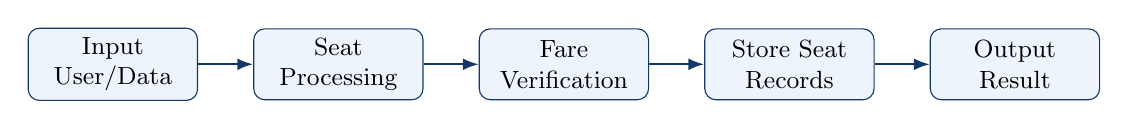
\begin{tikzpicture}[
node distance=7mm,
box/.style={rectangle,rounded corners,draw=GEUBlue,fill=GEULightBlue,
minimum width=2.15cm,minimum height=9mm,align=center,font=\small},
arrow/.style={-{Latex[length=2mm]},thick,draw=GEUBlue}
]
\node[box] (a) {Input\\User/Data};
\node[box,right=of a] (b) {Seat\\Processing};
\node[box,right=of b] (c) {Fare\\Verification};
\node[box,right=of c] (d) {Store Seat\\Records};
\node[box,right=of d] (e) {Output\\Result};
\draw[arrow] (a)--(b); \draw[arrow] (b)--(c); \draw[arrow] (c)--(d); \draw[arrow] (d)--(e);
\end{tikzpicture}
\end{center}
\vspace{5mm}
\begin{columns}[T,totalwidth=\textwidth]
\column{.48\textwidth}
\textbf{\color{GEUBlue}Major Components}
\begin{itemize}\itemsep2pt
\item \placeholder{Seat Occupancy Detection}
\item \placeholder{Fare Verification}
\item \placeholder{Driver Status \& Departure}
\end{itemize}
\column{.48\textwidth}
\textbf{\color{GEUBlue}Data / Control Flow}
\begin{itemize}\itemsep2pt
\item \placeholder{Seat occupancy is detected.}
\item \placeholder{Fare Verification Module updates the seat status for the Driver Control Module.}
\item \placeholder{Seat status is verified and departure decision is made.}
\end{itemize}
\end{columns}
\end{frame}

% 8
\begin{frame}{Technology Stack \& Methodology}
\begin{columns}[T,totalwidth=\textwidth]
\column{.48\textwidth}
\begin{block}{Technology Stack}
\begin{itemize}\itemsep2pt
\item Programming: \placeholder{C++}
\item Database: \placeholder{PostgreSQL}
\item Tools / Framework: \placeholder{C++ STL}
\item IDE: \placeholder{Visual Studio Code}
\item Version Control: \placeholder{Git / GitHub}
\end{itemize}
\end{block}
\column{.48\textwidth}
\begin{block}{Development Methodology}
\begin{enumerate}\itemsep2pt
\item\placeholder{Requirement Analysis} 
\item\placeholder{System Design}
\item\placeholder{Implementation} 
\item\placeholder{Testing} 
\item\placeholder{Evaluation} 
\end{enumerate}
\end{block}
\end{columns}
\vfill
\begin{center}
    \scriptsize
    \textbf{\color{GEUBlue}Justification:}\placeholder{C++ supports OOP and data structures; MySQL enables data storage; 
    Git/GitHub supports collaboration and the methodology ensures systematic development.}
\end{center}
\end{frame}
% % 9
% 9
\begin{frame}{Initial Progress \& Team Contribution}
\begin{columns}[T,totalwidth=\textwidth]
\column{.44\textwidth}
\textbf{\color{GEUBlue}Progress Achieved}
\begin{itemize}\itemsep3pt
\item \placeholder{DSA concepts and literature study completed}
\item \placeholder{Identified core requirements}
\item \placeholder{System architecture designed}
\item \placeholder{OOP and seat modules initiated}
\item \placeholder{Prepared test datasets}
\end{itemize}
\column{.52\textwidth}
\textbf{\color{GEUBlue}Individual Contribution}
\vspace{2mm}
\scriptsize
\begin{tabularx}{\textwidth}{@{}p{1.8cm}|p{2.0cm}|X@{}}
\toprule
Member & Role & Contribution\\
\midrule
\placeholder{Karnika Jain} & \placeholder{Lead} & \placeholder{System Architecture, OOP Design, Seat Occupancy Detection}\\
\hline
\placeholder{Anirudh Bahuguna} & \placeholder{Developer} & \placeholder{Fare Verification, CardVerifier, Verification Logic}\\
\hline
\parbox[t]{1.8cm}{\placeholder{Aaditya}\\[-1pt]\placeholder{Budakoti}}
&
\parbox[t]{2.0cm}{\placeholder{DB/Testing}}
&
\placeholder{Data Management, State Validation, System Testing}\\
\hline
\placeholder{Aparajita Pant} & \placeholder{Developer/Docs} & \placeholder{Departure Decision, Driver Status Panel, System Integration}\\
\bottomrule
\end{tabularx}
\end{columns}
\end{frame}

% 10
\begin{frame}{Roadmap, Expected Outcomes \& References}
\begin{columns}[T,totalwidth=\textwidth]
\column{.47\textwidth}
\textbf{\color{GEUBlue}Roadmap}
\begin{enumerate}\itemsep3pt
\item Phase-I: Proposal \& System Design
\item Phase-II: C++ Development \& Module Implementation
\item Phase-III: Integration, Testing \& Final Demonstration
\end{enumerate}
\vspace{-1mm}
\textbf{\color{GEUBlue}Expected Outcomes}
\begin{itemize}\itemsep2pt
\item {\makebox[\linewidth][l]{\placeholder{Functional seat-level bus fare verification prototype.}}}
\item {\makebox[\linewidth][l]{\placeholder{Real-time tracking of seat occupancy and verification status.}}}
\item {\makebox[\linewidth][l]{\placeholder{ Driver-facing seat status panel with clear state indication.}}}
\item {\makebox[\linewidth][l]{\placeholder{Demonstration of OOP and DSA concepts in C++.}}}
\end{itemize}
\column{.60\textwidth}
\textbf{\color{GEUBlue}References}
\begin{enumerate}\itemsep3pt
\item \placeholder{Comparison and Evaluation of Fare Collection Technologies in Public Transport}
\item \placeholder{The C++ Standard Library}
\item \placeholder{PostgreSQL Documentation — Official Reference Manual.}
\item \placeholder{GitHub Repository — TapNGo Project}
\end{enumerate}
\vfill
\vspace{10mm}
\hfill
\colorbox{GEUBlue}{%
    \parbox{.50\textwidth}{%
        \centering
        \color{white}
        \textbf{Thank You}\\
        Questions \& Suggestions
    }%
}
\end{columns}
\end{frame}

\end{document}
